% Primary source: https://arxiv.org/abs/1710.10903
\documentclass[tikz,border=5pt]{standalone}
\usepackage[T1]{fontenc}
\usepackage{lmodern,amsmath,amssymb}
\usetikzlibrary{arrows.meta,calc,positioning,fit,backgrounds,shapes.geometric,matrix,decorations.pathreplacing,patterns}
\definecolor{ink}{gray}{0.08}
\definecolor{wash}{gray}{0.965}
\definecolor{soft}{gray}{0.45}
\tikzset{box/.style={draw=ink,line width=.65pt,fill=white,align=center,inner sep=4pt,outer sep=0pt,font=\small},flow/.style={draw=ink,line width=.65pt,-{Latex[length=1.8mm,width=1.3mm]},rounded corners=2pt},annotation/.style={font=\scriptsize,text=soft,align=center},groupbox/.style={draw=soft,dashed,line width=.45pt,fill=wash}}
\begin{document}
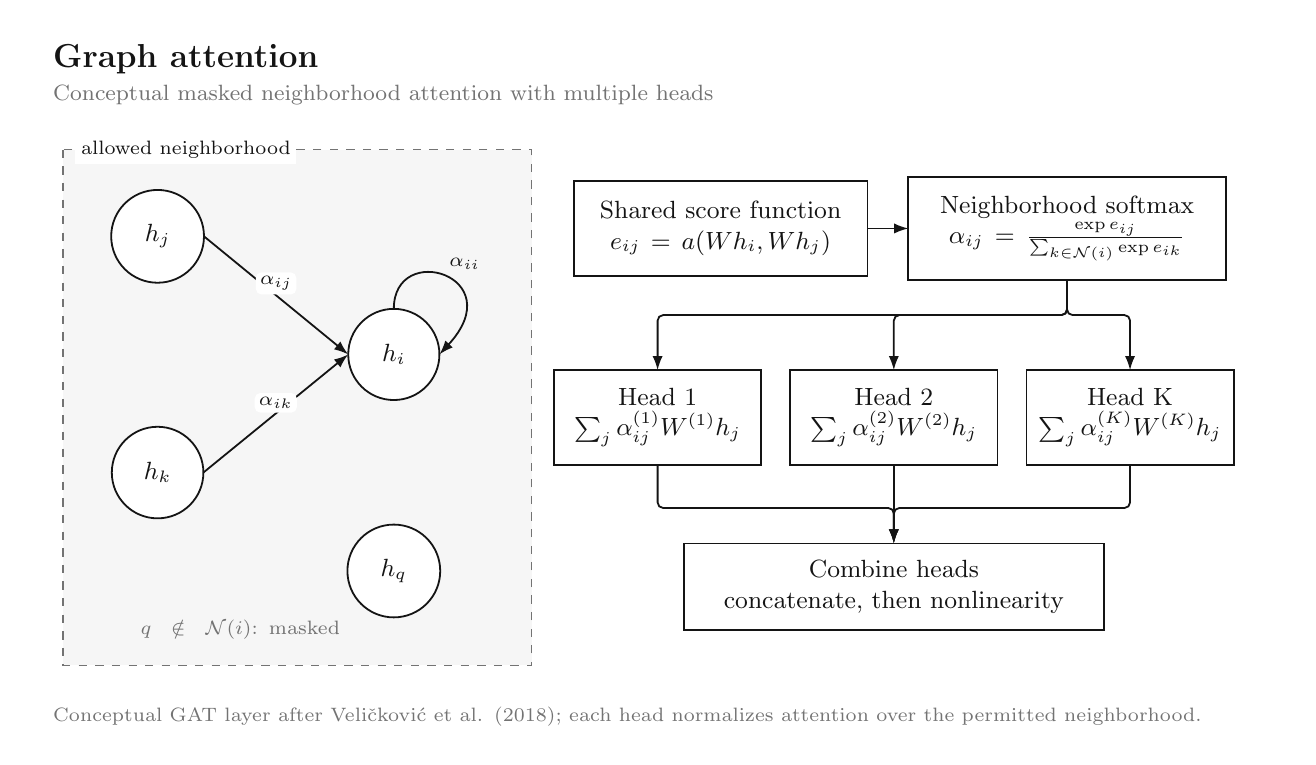
\begin{tikzpicture}[x=1cm,y=-1cm,font=\rmfamily,text=ink]

\path[use as bounding box] (0,0) rectangle (16,9);
\node[anchor=west,font=\large\bfseries] at (.2,.4) {Graph attention};
\node[anchor=west,font=\footnotesize,text=soft] at (.2,.85) {Conceptual masked neighborhood attention with multiple heads};
\begin{pgfonlayer}{background}
\draw[groupbox] (0.45,1.55) rectangle (6.4,8.1);
\node[anchor=west,font=\scriptsize,fill=white,inner sep=2pt] at (0.6,1.55) {allowed neighborhood};
\end{pgfonlayer}
\node[box,circle,minimum width=1.0cm,minimum height=1.0cm,text width=0.75cm] (u1) at (1.65,2.65) {$h_j$};
\node[box,circle,minimum width=1.0cm,minimum height=1.0cm,text width=0.75cm] (u2) at (1.65,5.65) {$h_k$};
\node[box,circle,minimum width=1.0cm,minimum height=1.0cm,text width=0.75cm] (target) at (4.65,4.15) {$h_i$};
\node[box,circle,minimum width=1.0cm,minimum height=1.0cm,text width=0.75cm] (excluded) at (4.65,6.9) {$h_q$};
\node[box,minimum width=3.7cm,minimum height=1.2cm,text width=3.45cm] (scores) at (8.8,2.55) {Shared score function\\$e_{ij}=a(Wh_i,Wh_j)$};
\node[box,minimum width=4.0cm,minimum height=1.3cm,text width=3.75cm] (softmax) at (13.2,2.55) {Neighborhood softmax\\$\alpha_{ij}=\frac{\exp e_{ij}}{\sum_{k\in\mathcal{N}(i)}\exp e_{ik}}$};
\node[box,minimum width=2.6cm,minimum height=1.2cm,text width=2.35cm] (head1) at (8.0,4.95) {Head 1\\$\sum_j\alpha^{(1)}_{ij}W^{(1)}h_j$};
\node[box,minimum width=2.6cm,minimum height=1.2cm,text width=2.35cm] (head2) at (11.0,4.95) {Head 2\\$\sum_j\alpha^{(2)}_{ij}W^{(2)}h_j$};
\node[box,minimum width=2.6cm,minimum height=1.2cm,text width=2.35cm] (headk) at (14.0,4.95) {Head K\\$\sum_j\alpha^{(K)}_{ij}W^{(K)}h_j$};
\node[box,minimum width=5.3cm,minimum height=1.1cm,text width=5.05cm] (combine) at (11.0,7.1) {Combine heads\\concatenate, then nonlinearity};
\begin{pgfonlayer}{background}
\draw[flow] (u1.east) -- (target.west) node[midway,above,fill=white,inner sep=1.5pt,font=\scriptsize] {$\alpha_{ij}$};
\draw[flow] (u2.east) -- (target.west) node[midway,above,fill=white,inner sep=1.5pt,font=\scriptsize] {$\alpha_{ik}$};
\draw[flow] (scores.east) -- (softmax.west);
\draw[flow] (softmax.south) -- (13.2,3.65) -- (8.0,3.65) -- (head1.north);
\draw[flow] (softmax.south) -- (13.2,3.65) -- (11.0,3.65) -- (head2.north);
\draw[flow] (softmax.south) -- (13.2,3.65) -- (14.0,3.65) -- (headk.north);
\draw[flow] (head1.south) -- (8.0,6.1) -- (11.0,6.1) -- (combine.north);
\draw[flow] (head2.south) -- (11.0,6.1) -- (11.0,6.1) -- (combine.north);
\draw[flow] (headk.south) -- (14.0,6.1) -- (11.0,6.1) -- (combine.north);
\end{pgfonlayer}
\draw[flow] (target.north) .. controls (4.65,2.7) and (6.15,3.15) .. (target.east);
\node[font=\scriptsize,fill=wash,inner sep=1pt] at (5.55,3.0) {$\alpha_{ii}$};
\node[annotation,text width=4.9cm] at (2.7,7.65) {$q\notin\mathcal{N}(i)$: masked};
\node[anchor=west,align=left,font=\scriptsize,text=soft,text width=15.6cm] at (.2,8.75) {Conceptual GAT layer after Veli\v{c}kovi\'c et al. (2018); each head normalizes attention over the permitted neighborhood.};
\end{tikzpicture}
\end{document}
